\documentclass[aspectratio=1610,14pt]{beamer}

\usepackage[utf8]{inputenc}
\usepackage{graphicx}
\usepackage{url}
\usepackage{minted}
\usepackage[absolute,overlay]{textpos}
\usepackage{tikz}

\graphicspath{{images/}}

\usetheme{csctraining}

\usemintedstyle{emacs}
\definecolor{codebg}{rgb}{0.95,0.95,0.95}
\definecolor{codehl}{rgb}{0.95,0.95,0.05}
\setminted{highlightcolor=codehl,bgcolor=codebg}

\newcommand{\link}[1]{\alert{\url{#1}}}
\newcommand{\vitem}{\vfill\item}

\title{Machine Learning\\on Puhti}
\subtitle{Part 2: Scaling up and using resources efficiently\\[5mm]
  June 10, 2020\\
  Mats Sjöberg\\
  {\tt mats.sjoberg@csc.fi}}

\begin{document}

\begin{frame}{Webinar: Machine Learning on Puhti}
  \begin{columns}[t]
    \begin{column}{0.45\linewidth}
      \vfill
      \hspace{15mm} {\em Wed, June 3} \\[5mm]

      \textbf{Part 1: Getting started}
      
      \begin{itemize}
      \item CSC's services
      \item Puhti supercomputer
      \item Available software
      \item Running jobs on Puhti
      \item Data storage
      \end{itemize}
    \end{column}
    \begin{column}{0.55\linewidth}
      \vfill
      \hspace{12mm} \alert{\em TODAY} \\[5mm]
      
      \textbf{Part 2: Scaling up and using resources efficiently}
      
      \begin{itemize}
      \item Efficient data storage
      \item GPU utilization
      \item Multi-GPU and multi-node jobs
      \item Singularity containers
      \end{itemize}
    \end{column}
  \end{columns}
  \vspace{10mm}
  \link{https://github.com/csc-training/ml-webinar/}
\end{frame}

\section{Efficient data storage}

\begin{frame}{Data storage on Puhti}

  \begin{itemize}
  \item Disk space and \emph{number of files} are limited on Puhti! \\
    {\small $\rightarrow$ We want to ensure that the shared (Lustre) filesystem works
    efficiently for everyone!}
  \item Useful command: {\tt csc-workspaces}
  \end{itemize}

  \vfill

  {\footnotesize
    \begin{tabular}{lllrrl}
             & Owner    & Path                      & Capacity & Number of files & Cleaning \\
    \hline
    home     & Personal & {\tt /users/<user-name>}  & 10 GiB   & 100 000 files   & No \\
    projappl & Project  & {\tt /projappl/<project>} & 50 GiB   & 100 000 files   & No \\
    scratch  & Project  & {\tt /scratch/<project>}  & 1 TiB    & 1 000 000 files & Yes - 90 days \\
    \end{tabular}
  }
  \vfill
  {\small
    Data quotas can be increased via MyCSC!

    \link{https://docs.csc.fi/computing/disk/}}
\end{frame}

\begin{frame}[fragile]{Using Allas}
  \begin{itemize}
  \item store big datasets in Allas, CSC's object storage
  \item download them to project scratch prior to computation
  \item you can also upload trained models (or keep in projappl)
  \end{itemize}

  \vfill
  
  % \begin{verbatim}
\begin{minted}{shell-session}
$ module load allas
$ allas-conf
$ cd /scratch/<your-project>
$ swift download <bucket-name> your-dataset.tar  
\end{minted}
%\end{verbatim}
\end{frame}

\begin{frame}{Large number of files}
  \begin{itemize}
  \vitem Many datasets contain a large number of small files
  \vitem Shared filesystem (Lustre) performs poorly in this scenario \\
    $\rightarrow$ noticable slowdowns for all Puhti users!
  \end{itemize}

  \vfill
  Consider alternatives:

  \begin{itemize}
  \vitem packaging your dataset into larger files                     
  \vitem use NVME fast local storage on GPU nodes
  \end{itemize}
\end{frame}

\begin{frame}{Using more efficient data formats}

  Instead of many small files, use one or a few bigger files.

  \vfill
  
  Examples:

  \begin{itemize}
  \vitem TensorFlow's TFRecord format
  \vitem HDF5
  \vitem LMDB
  \vitem ZIP, for example via Python's {\tt zipfile} library
  \end{itemize}

  \vfill
\end{frame}

\begin{frame}[fragile]{Fast local NVME drive}

  \begin{itemize}
  \item All GPU nodes have a local NVME drive
  \item Just add {\tt nvme:<number-of-GB>} to sbatch {\tt --gres} flag
  \end{itemize}

\begin{minted}[fontsize=\footnotesize,highlightlines={8,10,12}]{bash}
#!/bin/bash
#SBATCH --account=<project>
#SBATCH --partition=gpu
#SBATCH --ntasks=1
#SBATCH --cpus-per-task=10
#SBATCH --mem=64G
#SBATCH --time=1:00:00
#SBATCH --gres=gpu:v100:1,nvme:100

tar xf /scratch/<your-project>/your-dataset.tar -C $LOCAL_SCRATCH

srun python3 myprog.py --data_dir=$LOCAL_SCRATCH <options>
\end{minted}

\end{frame}

\section{GPU utilization}

\begin{frame}{GPU utilization}

GPUs are an expensive resource compared to CPUs ($\times$ 60 BUs!) \\
$\rightarrow$ GPU should be maximally utilized!

\vspace{1em}

\begin{minipage}{0.8\textwidth}
For a running job:
\begin{itemize}
\item use {\tt squeue} to find out on what node (computer) it is running
\item ssh into that node, e.g., {\tt ssh r01g01}
\item run {\tt nvidia-smi}
\end{itemize}
\end{minipage}

\begin{textblock}{6}(9.8,8)
  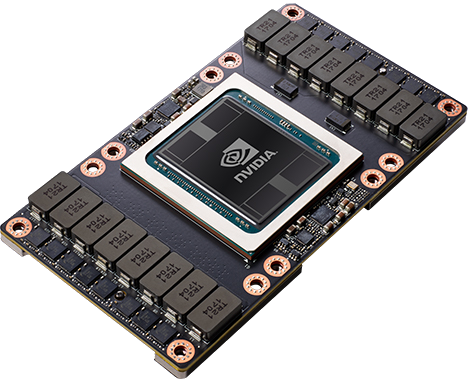
\includegraphics[width=\textwidth]{v100}
\end{textblock}
\end{frame}

\begin{frame}{GPU utilization}

  For a finished job:

  \begin{itemize}
  \vitem run {\tt gpuseff <jobid>}
  \vitem shows GPU utilization statistics for the whole running time
  \vitem \alert{note:} gpuseff is currently in testing usage, and still
    under development
  \end{itemize}

  \vfill
  
  You can always contact our service desk if you need advice on how to
  improve your GPU utilization!
\end{frame}

\begin{frame}[fragile]{Using multiple CPUs for ETL}
  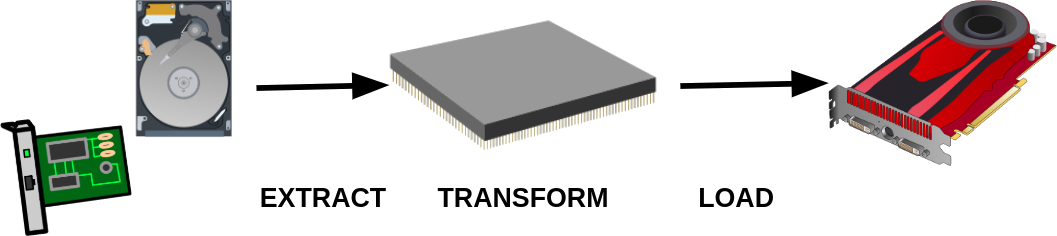
\includegraphics[width=\textwidth]{etl}

  \begin{itemize}
  \item Common bottle-neck: CPU cannot keep up with GPU
  \item GPU has to wait for more data \ldots
  \item Solution: use more CPUs (they are ``cheaper'' than GPUs!)
  \end{itemize}

  \vspace{0.5em}
  
  A good \alert{rule of thumb in Puhti is to reserve 10 CPUs per GPU} \\
  (as there are 4 GPUs and 40 CPUs per node).

\end{frame}

\begin{frame}[fragile]{Using multiple CPUs for ETL}
  In Slurm scripts:
\begin{minted}{bash}
#SBATCH --cpus-per-task=10
\end{minted}

\vspace{0.5em}

\alert{Note:} using multiple CPUs \emph{not} automatic, code needs to support it!

\vspace{0.5em}

  For example in TensorFlow:

\begin{minted}[fontsize=\small]{python}
dataset = dataset.map(..., num_parallel_calls=10)
dataset = dataset.prefetch(buffer_size)
\end{minted}

  PyTorch:

\begin{minted}[fontsize=\small]{python}
train_loader = torch.utils.data.DataLoader(..., num_workers=10)
\end{minted}
\end{frame}

\section{Multi-GPU and multi-node jobs}

\begin{frame}[fragile]{Multi-GPU}

  Many frameworks support multi-GPU within a single node.

  \vspace{0.5em}
  
  Slurm script:
  \begin{minted}{bash}
#SBATCH --gres=gpu:v100:4
  \end{minted}

  \vspace{0.5em}
  
  \begin{columns}[t]
    \begin{column}{0.47\linewidth}
      TensorFlow:
      
      \begin{minted}[fontsize=\footnotesize]{python}
mirrored_strategy = \
  tf.distribute.MirroredStrategy()
with mirrored_strategy.scope():
    model = Sequential(...)
    model.add(...)
    model.add(...)
    model.compile(...)
      \end{minted}
    \end{column}
    \begin{column}{0.47\linewidth}
      PyTorch:
      
      \begin{minted}[fontsize=\footnotesize]{python}
model = MyModel(...)
if torch.cuda.device_count() > 1:
    model = nn.DataParallel(model)
model.to(device)
      \end{minted}
    \end{column}
  \end{columns}
\end{frame}

\begin{frame}[fragile]{Multi-GPU and multi-node}
  \begin{itemize}
  \item If you need more than 4 GPUs, we recommend \alert{Horovod}
  \item Supported for TensorFlow and PyTorch on Puhti
  \item Uses MPI and NCCL2 for interprocess communication
  \item Also requires some changes in the code, see e.g.: \\
    {\small \link{https://github.com/horovod/horovod/tree/master/examples}}
  \item In Puhti modules with {\tt -hvd} suffix are Horovod-enabled
  \end{itemize}

  \vspace{0.7em}

  Try: \vspace{-2mm}
\begin{verbatim}
module avail hvd
module load tensorflow/2.0.0-hvd
\end{verbatim}
\end{frame}

\begin{frame}[fragile]{Slurm example for Horovod}
  Example slurm script that uses \alert{8 GPUs} across \alert{two computers}

\begin{itemize}
\item MPI terminology: 8 tasks, 2 nodes
\item Each task is 1 GPU and 10 CPUs
\end{itemize}
  
  \begin{minted}[fontsize=\small,highlightlines={4,5,6,8}]{bash}
#!/bin/bash
#SBATCH --account=<project>
#SBATCH --partition=gpu
#SBATCH --ntasks=8
#SBATCH --nodes=2
#SBATCH --cpus-per-task=10
#SBATCH --mem=32G
#SBATCH --time=1:00:00
#SBATCH --gres=gpu:v100:4

srun python3 myprog.py <options>
\end{minted}
\end{frame}

% srun --ntasks=$SLURM_NNODES --ntasks-per-node=1 \
%     tar xf /scratch/<your-project>/your-dataset.tar -C $LOCAL_SCRATCH  

\section{Singularity containers}

\begin{frame}[fragile]{Singularity on Puhti}
  \begin{itemize}
  \item Puhti supports Singularity-based containers
  \item Some of our modules use it -- just remember to prefix commands with \
    {\tt singularity\_wrapper exec}
  \item You can also convert your own Docker containers, see:
    {\small \link{https://docs.csc.fi/computing/containers/run-existing/}}
  \end{itemize}

  \vspace{5mm}
  Conversion (preferrably not in login nodes!):
  \vspace{-4mm}
\begin{minted}[fontsize=\small]{shell-session}
$ singularity build pytorch_20.03-py3.sif \
              docker://nvcr.io/nvidia/pytorch:20.03-py3
\end{minted}

Extract from Slurm script:
\vspace{-4mm}
\begin{minted}[fontsize=\small]{bash}
srun singularity_wrapper exec --nv pytorch_20.03-py3.sif \
    python3 myprog <options>
\end{minted}
  
\end{frame}

\begin{frame}[fragile]{Special Singularity-based applications}

  Specialized Singularity-based applications not shown with default modules

  \vspace{1em}

  \alert{Example:} Turku neural parser

\begin{minted}[fontsize=\small]{shell-session}
$ module use /appl/soft/ai/singularity/modulefiles/
$ module load turku-neural-parser/fi-en-sv-gpu
$ echo "Minulla on koira." | singularity_wrapper run \
    stream fi_tdt parse_plaintext
\end{minted}
  
\end{frame}

\begin{frame}{Further resources}
  \begin{itemize}
  \item Accessing and using Puhti: \link{https://docs.csc.fi/computing/overview/}
  \item MyCSC portal: \link{https://my.csc.fi}
  \item Machine learning software on Puhti: \\
    {\footnotesize \link{https://docs.csc.fi/apps/\#data-analytics-and-machine-learning}}
  \item GPU-accelerated machine learning guide: \link{https://docs.csc.fi/support/tutorials/gpu-ml/}
  \item Slides and code from this webinar: \link{https://github.com/csc-training/ml-webinar/}
  \item Deploying machine learning on Rahti: \link{https://github.com/cscfi/rahti-ml-examples}
  \end{itemize}
\end{frame}

\section*{Thank you!}

\end{document}

%%% Local Variables: 
%%% TeX-command-extra-options: "-shell-escape"
%%% End:
